\subsection{Security Assessment}

The initial step of security assessment required identifying assets. We concluded that our assets consisted of both software and infrastructure resources. Subsequently, we identified threat sources to be hackers, cybercriminals, insiders, competitors (other groups), and the environment. Next, we went on and created risk scenarios based on OWASP's top 10 vulnerabilities for 2021, and other sources based on personal experience. Finally, we assessed their impact and likelihood (Figure~\ref{fig:securityAssessment}). Based on that, we performed some actions to mitigate the biggest risks, for instance, deleted secrets exposed in our repository as well as closed exposed but unused ports in our services.

\begin{figure}[h]
\centering
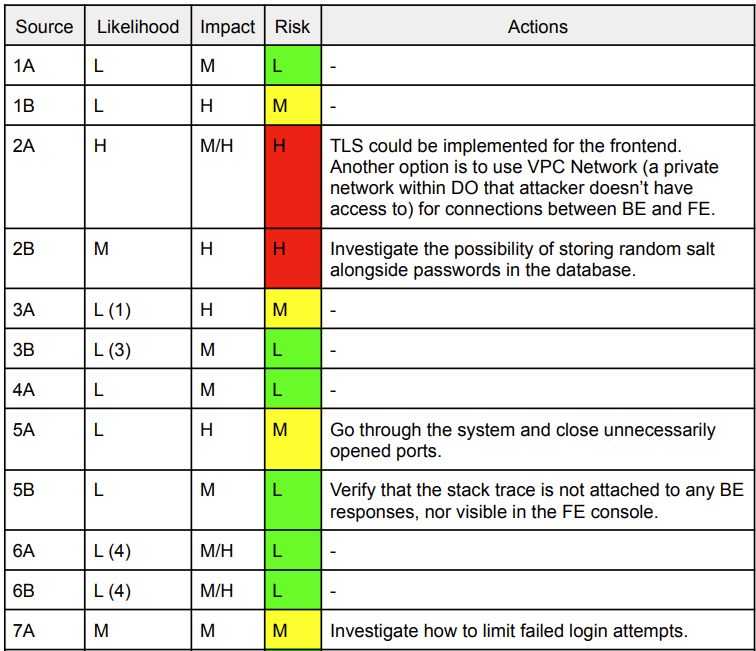
\includegraphics[width=0.5\textwidth]{images/SecurityAssessmentSnapshot.png}
\caption{A snapshot of security assessment table~\cite{securityAssessment}.}
\label{fig:securityAssessment}
\end{figure}